% !TEX root = ../Main.tex
\chapter{特殊垂直结构的外接球}

除了正多面体与长方体模型外，高考还常见\textbf{含"垂直"结构}的立体外接球题型。本章整理几类：侧棱垂直底面、侧面垂直底面、两侧面互垂直。统一策略：\textbf{找一个"好"面 $\to$ 过外接圆圆心作垂线 $\to$ 球心必在此垂线上 $\to$ 代入距离方程}。

\section{一侧棱垂直于底面}

\state{模型：$PC \perp$ 底面 $\triangle ABC$}{
    若三棱锥 $P$-$ABC$ 中 $PC \perp$ 平面 $ABC$，则 $PC$ 是\textbf{外接球的一条弦}（弦指球面上两点连线段）。

    \textbf{球心定位}：过 $\triangle ABC$ 外接圆圆心 $O_1$ 作底面垂线 $\ell_1$；过 $PC$ 的中点 $M$ 作 $PC$ 的中垂面 $\alpha$。球心 $O$ 在 $\ell_1 \cap \alpha$——即 $O$ 在 $\ell_1$ 上且 $OM \perp PC$。
    设 $r$ 为 $\triangle ABC$ 外接圆半径、$PC = h$。由球心在 $\ell_1$ 上且与 $P, C$ 等距：
    \[
    R^2 = r^2 + \left(\frac{h}{2}\right)^2.
    \]
}

\begin{center}
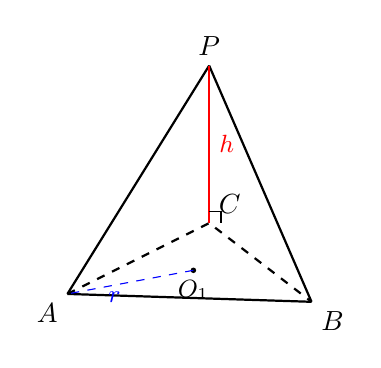
\begin{tikzpicture}[scale=1]
    \coordinate (A) at (-1.6,-0.5);
    \coordinate (B) at (1.5,-0.6);
    \coordinate (C) at (0.2, 0.4);
    \coordinate (P) at (0.2, 2.4);
    \draw[thick] (A) -- (B);
    \draw[thick, dashed] (A) -- (C) -- (B);
    \draw[thick] (P) -- (A);
    \draw[thick] (P) -- (B);
    \draw[thick, red] (P) -- (C) node[midway, right] {\small $h$};
    % foot-of-perpendicular marker
    \draw[thin] (0.2, 0.55) -- (0.35, 0.55) -- (0.35, 0.4);
    \coordinate (O1) at (0.0, -0.2);
    \fill (O1) circle (1pt) node[below] {\small $O_1$};
    \draw[dashed, blue] (O1) -- (A) node[midway, below left] {\small $r$};
    \node at (P) [above] {$P$};
    \node at (A) [below left] {$A$};
    \node at (B) [below right] {$B$};
    \node at (C) [above right] {$C$};
\end{tikzpicture}
\end{center}

\ex[侧棱垂直模型应用]{
    三棱锥 $S$-$ABC$ 所有顶点都在球 $O$ 面上，$SA \perp$ 平面 $ABC$，$SA = 2\sqrt 3, AB = 1, AC = 2, \angle BAC = \tfrac{\pi}{3}$。求球 $O$ 的表面积。
}

\sol{
    \textbf{底面 $\triangle ABC$ 外接圆半径。} 由余弦定理 $BC^2 = 1 + 4 - 2 \cdot 1 \cdot 2 \cdot \cos \tfrac{\pi}{3} = 3$，$BC = \sqrt 3$。正弦定理：
    \[
    \frac{BC}{\sin \angle BAC} = 2 r \implies r = \frac{\sqrt 3}{2 \cdot \sqrt 3/2} = 1.
    \]

    \textbf{用模型公式。} $SA$ 垂直底面，$SA = 2\sqrt 3$：
    \[
    R^2 = r^2 + \left(\frac{SA}{2}\right)^2 = 1 + 3 = 4, \qquad R = 2.
    \]

    \textbf{表面积} $= 4\pi R^2 = 16 \pi$。
}

\section{两侧面互相垂直}

\state{模型：平面 $PAC \perp$ 平面 $BAC$}{
    设两侧面 $\triangle PAC$ 与 $\triangle BAC$ 共一边 $AC$，且\textbf{两平面互相垂直}（记 $AC = l$、两三角形外接圆半径分别为 $r_1, r_2$，圆心 $O_1, O_2$）。

    球心定位：过 $O_1$ 作 $PAC$ 的垂线 $\ell_1$，过 $O_2$ 作 $BAC$ 的垂线 $\ell_2$。两线在空间中交于点——由\textbf{两平面垂直}，$\ell_1$ 在 $BAC$ 内，$\ell_2$ 在 $PAC$ 内，\textbf{两线交点恰为球心} $O$。

    \textbf{代数上：} $O_1$ 到 $AC$ 的距离为 $\sqrt{r_1^2 - (l/2)^2}$（由 $O_1$ 是 $\triangle PAC$ 外心到弦 $AC$ 距离）；同理 $O_2$ 到 $AC$ 的距离为 $\sqrt{r_2^2 - (l/2)^2}$。利用两平面垂直、$O, O_1, O_2$ 组成的直角三角形关系：
    \[
    R^2 = \left[r_1^2 - \left(\frac{l}{2}\right)^2\right] + \left[r_2^2 - \left(\frac{l}{2}\right)^2\right] + \left(\frac{l}{2}\right)^2 = r_1^2 + r_2^2 - \left(\frac{l}{2}\right)^2.
    \]
    \textbf{重要公式}：$\boxed{R^2 = r_1^2 + r_2^2 - (l/2)^2.}$
}

\ex[两侧面互垂直公式应用]{
    点 $A$ 是以 $BC$ 为直径的圆 $O$ 上异于 $B, C$ 的动点，$P$ 为平面 $ABC$ 外一点，平面 $PBC \perp$ 平面 $ABC$，$BC = 3, PB = 2\sqrt 2, PC = \sqrt 5$。求三棱锥 $P$-$ABC$ 外接球的表面积。
}

\sol{
    \textbf{两平面共边 $BC$、互相垂直}——正是上述模型。
    \textbf{共边长} $l = BC = 3$。

    \textbf{$\triangle ABC$ 外接圆半径 $r_1$}：由于 $BC$ 是圆 $O$ 的直径，$A$ 在此圆上，故 $\triangle ABC$ 的外接圆\textbf{就是}圆 $O$，半径 $r_1 = \tfrac{3}{2}$。

    \textbf{$\triangle PBC$ 外接圆半径 $r_2$}：$PB = 2\sqrt 2, PC = \sqrt 5, BC = 3$。$\cos \angle BPC = \dfrac{8 + 5 - 9}{2 \cdot 2\sqrt 2 \cdot \sqrt 5} = \dfrac{4}{4\sqrt{10}} = \dfrac{1}{\sqrt{10}}$，$\sin \angle BPC = \dfrac{3}{\sqrt{10}}$（由 $\sin^2 + \cos^2 = 1$）。正弦定理：
    \[
    r_2 = \frac{BC}{2 \sin \angle BPC} = \frac{3}{2 \cdot 3/\sqrt{10}} = \frac{\sqrt{10}}{2}.
    \]

    \textbf{套公式}：
    \[
    R^2 = \left(\frac{3}{2}\right)^2 + \left(\frac{\sqrt{10}}{2}\right)^2 - \left(\frac{3}{2}\right)^2 = \frac{10}{4} = \frac{5}{2}.
    \]
    表面积 $= 4\pi R^2 = 10 \pi$。
}

\section{两侧面为直角三角形、共斜边}

\state{模型：两直角三角形拼成的四面体}{
    若四面体 $P$-$ABC$ 中两侧面 $\triangle PAB, \triangle QAB$ 都是\textbf{以 $AB$ 为斜边}的直角三角形——即 $\angle APB = \angle AQB = 90^\circ$（这里笔记中的 $P, Q$ 是四面体的两个异于 $A, B$ 的顶点）。

    \textbf{关键观察}：直角 $\angle APB$ 意味 $P$ 在以 $AB$ 为直径的圆上；直角 $\angle AQB$ 意味 $Q$ 在以 $AB$ 为直径的圆上。故 $A, B, P, Q$ 都在以\textbf{$AB$ 为直径的球面}上——\textbf{$AB$ 就是外接球的直径}。
    \[
    \boxed{R = \frac{AB}{2}.}
    \]
}

\rmkb{
    \textbf{本章三个模型一览}：
    \begin{enumerate}
        \item \textbf{一侧棱 $\perp$ 底面}：$R^2 = r^2 + (h/2)^2$（$r$ = 底面外接圆半径，$h$ = 垂直棱长）；
        \item \textbf{两侧面互垂直、共边}：$R^2 = r_1^2 + r_2^2 - (l/2)^2$（$r_i$ = 两面外接圆半径，$l$ = 共边长）；
        \item \textbf{两侧面均为以共边为斜边的直角三角形}：$R = \dfrac{AB}{2}$——\textbf{共边就是直径}。
    \end{enumerate}

    \textbf{识别流程}：看到"垂直"关键词 $\to$ 判断是"棱 $\perp$ 面"、"面 $\perp$ 面"、还是"棱之间互垂直" $\to$ 选对应模型。
}
